\documentclass{article}

\usepackage{graphicx}
\usepackage{tikz}
\usepackage{tikzsymbols}
\usetikzlibrary{calc,patterns,shapes.geometric}
\pagestyle{empty}
\usepackage[margin=0pt]{geometry}
\geometry{papersize={14in,12in}}

\def\centerarc[#1](#2)(#3:#4:#5){\draw[#1] ($(#2)+({#5*cos(#3)},{#5*sin(#3)})$) arc (#3:#4:#5);}

\begin{document}
	\begin{figure}
		\centering
		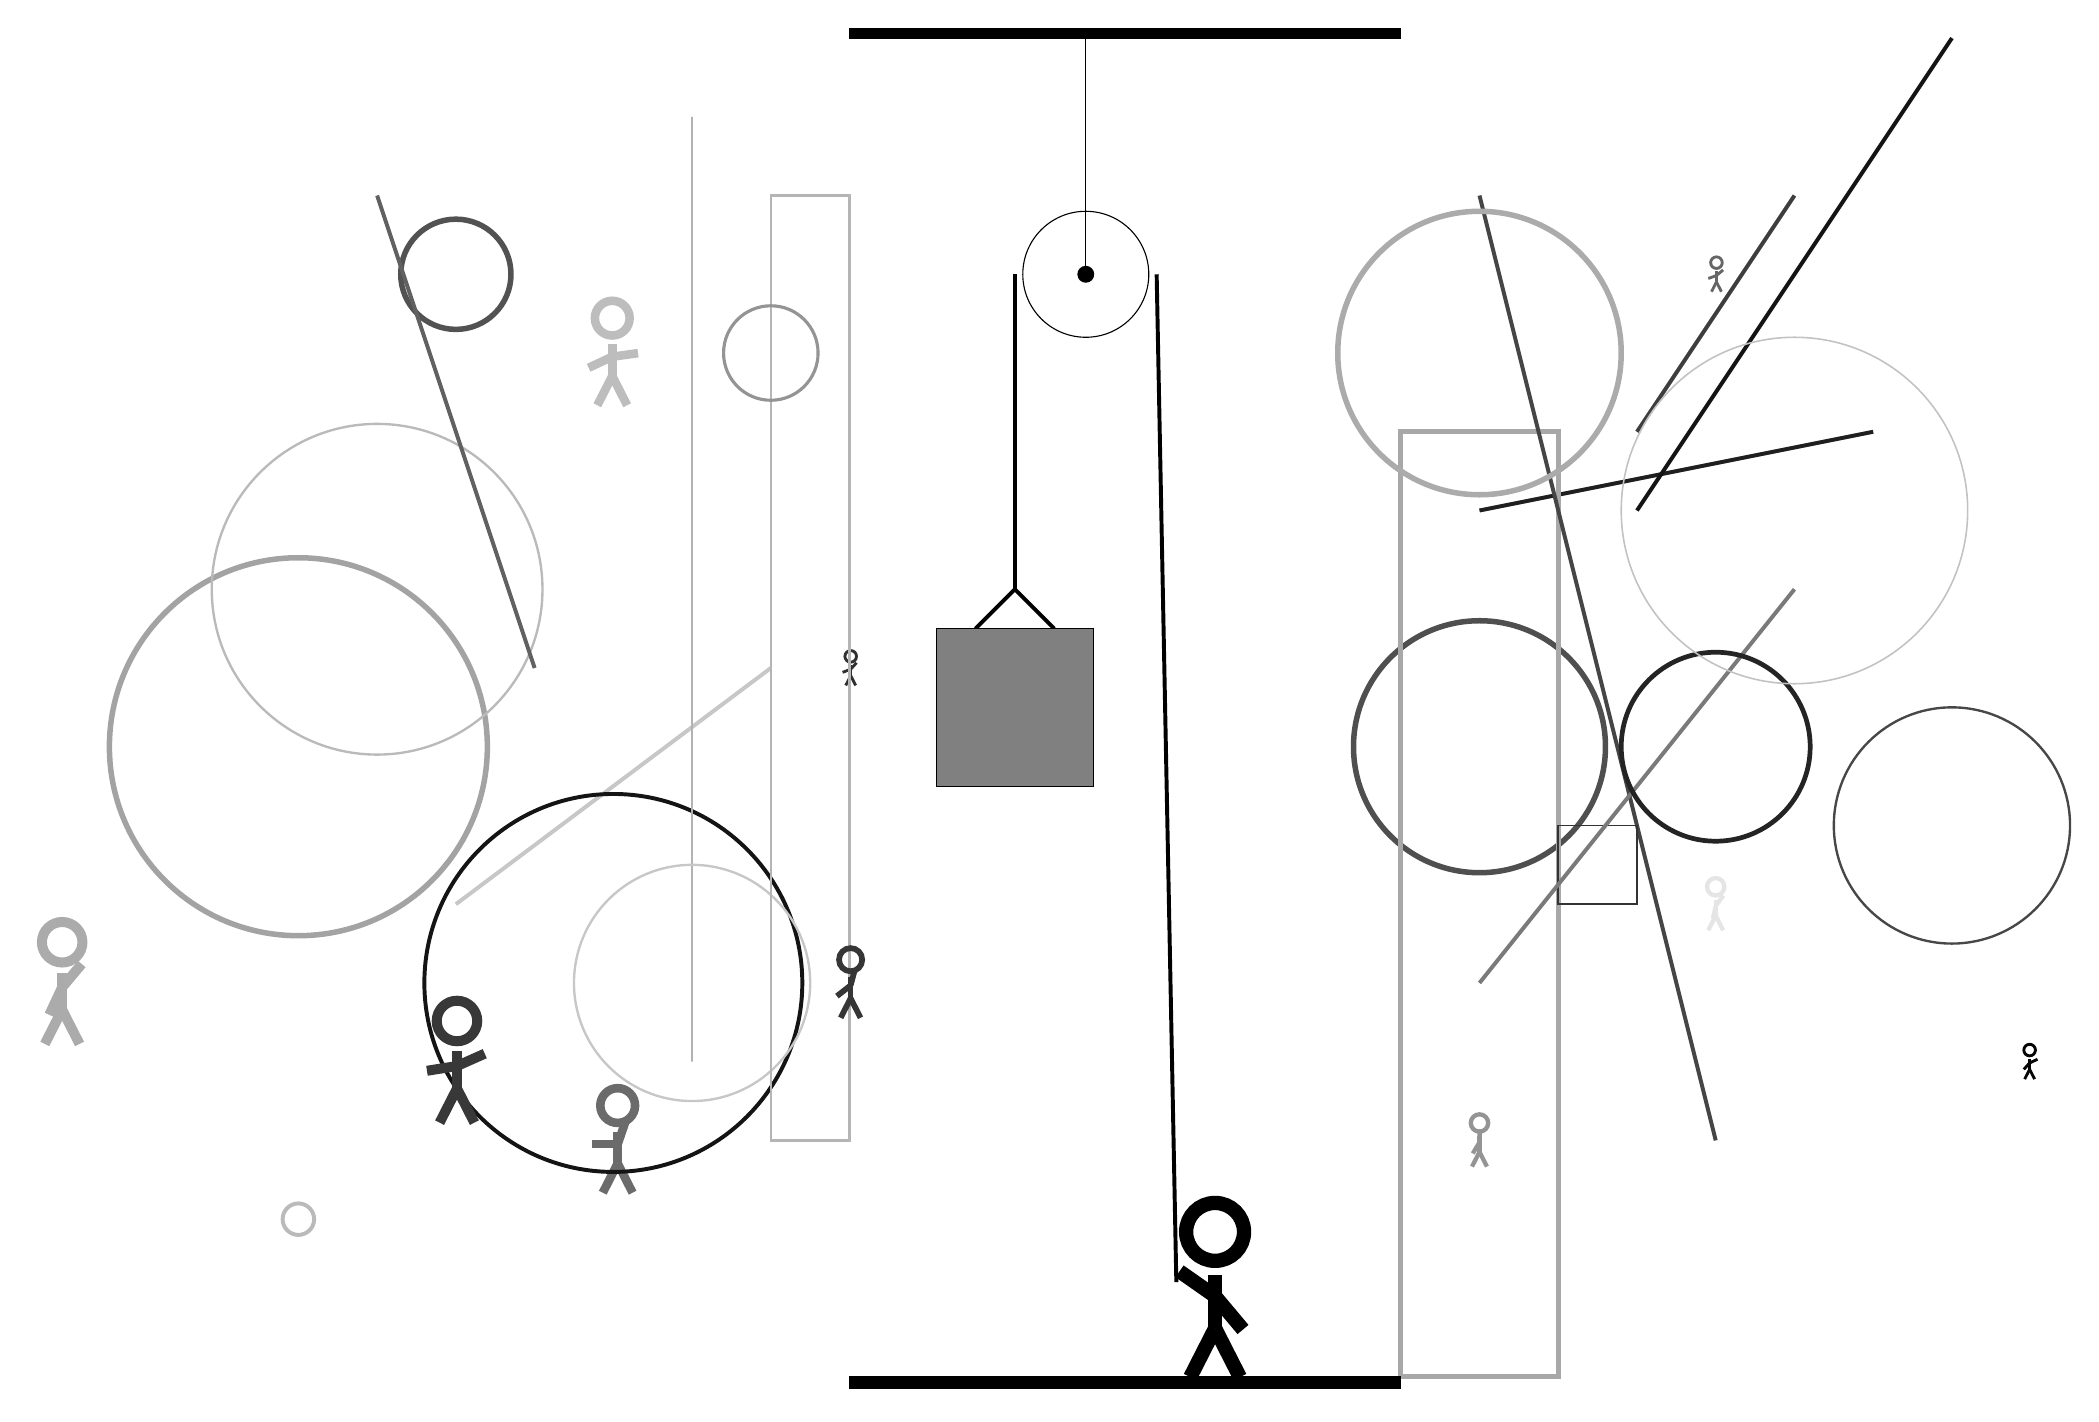
\begin{tikzpicture}
			%%%%% START %%%%%
			
			\draw[fill=black] (-2, 14) rectangle (5, 14.125);
			
			\draw (1, 11) circle (0.8);
			\draw[fill=black] (1, 11) circle (0.1);
			\draw (1, 14) -- (1, 11);
			
			\draw[line width=0.5mm] (-0.4, 6.5) -- (0.1, 7.0) -- (0.6, 6.5);
			\draw[fill=black!50] (-0.9, 6.5) rectangle (1.1, 4.5);
			
			\node[line width=0.7mm, color=black!58] at (-5, 0) {\Strichmaxerl[6][0][71]};
			
			\draw[line width=0.5mm, color=black!88](6, 8) -- (11, 9);
			\draw[line width=0.5mm, color=black!22](-7, 3) -- (-3, 6);
			\draw [line width=0.5mm, color=black!27](-9, -1) circle (0.2);
			\draw [line width=0.7mm, color=black!69](6, 5) circle (1.6);
			
			\draw [line width=0.7mm, color=black!68](-7, 11) circle (0.7);
			
			\draw[line width=0.6mm, color=black!34] (5, 9) rectangle (7, -3);
			\draw[line width=0.5mm, color=black!73](6, 12) -- (9, 0);
			\draw [line width=0.7mm, color=black!33](6, 10) circle (1.8);
			\draw [line width=0.5mm, color=black!92](-5, 2) circle (2.4);
			
			\draw[line width=0.5mm, color=black!76](8, 9) -- (10, 12);
			\draw [line width=0.7mm, color=black!36](-9, 5) circle (2.4);
			\draw [line width=0.3mm, color=black!72](12, 4) circle (1.5);
			\draw[line width=0.2mm, color=black!80] (7, 4) rectangle (8, 3);
			\draw[line width=0.2mm, color=black!30] (-4, 13) rectangle (-4, 1);
			\draw[line width=0.5mm, color=black!52](10, 7) -- (6, 2);
			\node[line width=0.6mm, color=black!33] at (-12, 2) {\Strichmaxerl[7][65][50]};
			
			\draw [line width=0.3mm, color=black!22](-4, 2) circle (1.5);
			\node[line width=0.4mm, color=black!10] at (9, 3) {\Strichmaxerl[3][77][54]};
			\node[line width=0.7mm, color=black!26] at (-5, 10) {\Strichmaxerl[6][25][8]};
			\draw[line width=0.5mm, color=black!92](8, 8) -- (12, 14);
			
			\node[line width=0.5mm, color=black!81] at (-2, 6) {\Strichmaxerl[2][21][48]};
			
			\node[line width=0.2mm, color=black!78] at (-7, 1) {\Strichmaxerl[7][9][24]};
			\draw [line width=0.6mm, color=black!86](9, 5) circle (1.2);
			\draw[line width=0.3mm, color=black!29] (-3, 12) rectangle (-2, 0);
			\node[line width=0.4mm, color=black!79] at (-2, 2) {\Strichmaxerl[4][38][75]};
			\draw [line width=0.4mm, color=black!42](-3, 10) circle (0.6);
			\draw [line width=0.3mm, color=black!27](-8, 7) circle (2.1);
			\node[line width=0.6mm, color=black!60] at (9, 11) {\Strichmaxerl[2][20][40]};
			\node[line width=0.3mm, color=black!98] at (13, 1) {\Strichmaxerl[2][48][25]};
			\draw [line width=0.2mm, color=black!24](10, 8) circle (2.2);
			\node[line width=0.4mm, color=black!42] at (6, 0) {\Strichmaxerl[3][59][89]};
			\draw[line width=0.5mm, color=black!62](-6, 6) -- (-8, 12);
			
			
			\draw[line width=0.5mm] (0.1, 11) -- (0.1, 7.0);
			\centerarc[line width=0.5mm](1, 11)(0:180:0.9);
			\draw[line width=0.5mm](1.9, 11) -- (2.15, -1.8);
			
			\node at (2.6, -1.9) {\Strichmaxerl[10][-35][-50]};
			
			\draw[fill=black] (-2, -3) rectangle (5, -3.15);
			
			%%%%% END %%%%%
		\end{tikzpicture}
	\end{figure}	
\end{document}